% Provenance (never printed): see sources/outline_sources.md (Year 2: ore deposits ---
% magmatic, hydrothermal, sedimentary and supergene deposits; grade and tonnage; exploration).
% Deposit descriptions from the USGS Mineral Deposit Models for Resource Assessment
% (Scientific Investigations Report 2010-5070, chapters A, B, C, E, I, L, N, O, Q), USGS
% Open-File Report 03-077 (orogenic gold) and Grabreck et al. 2022 (kimberlites); the grade and
% tonnage data of the world's porphyry copper deposits from USGS Open-File Report 2008-1155
% (dataset bachelor-2-porphyry-cu). Ledger rows in sources/ledger/book4.md; curves and numbers
% from figdata/bachelor-2/ores.py and the Book 4 second-writer scratch calculator calc/ch29.py.
% Geology and sourced numbers only: no advocacy.
\chapter{Ertsafzettingen}\label{ch:b2:ore-deposits}

Koper maakt ongeveer \qty{0.006}{\percent} van de korst uit; het wordt gewonnen uit gesteente dat ongeveer
\qty{0.5}{\percent} bevat. Elke kopermijn ligt dus op gesteente dat zo'n tachtig keer rijker is dan de
korst eromheen, en elke \omterm{def:b2:ore-deposits:deposit}{ertsafzetting} is het werk van een natuurlijke concentrator: een \omterm{def:b2:magma-emplacement:magma}{magma} waaruit
een sulfidesmelt ontmengde, een hete pekel die metalen oploste en in een spleet afzette, een
rivier die zware korrels van lichte scheidde, regen die de top van een ertslichaam uitloogde en
het koper ervan dieper weer afzette. Dit hoofdstuk volgt deze concentratoren, meet daarna hun
producten --- hoeveel erts, met welk gehalte --- en eindigt met de manier waarop afzettingen worden gevonden.
% ledger: perkins:ore-grades

\begin{recall}
\textbf{Uit de schoolboeken}: \omterm{def:b2:ore-deposits:deposit}{ertsafzetting} en \omterm{def:b2:ore-deposits:cf}{concentratiefactor}, ader, \omterm{def:b2:ore-deposits:placer}{placer}, reserve en
voorraad; hydrothermale circulatie en zwarte rokers op ruggen. \textbf{Uit de
scheikundeboeken}: erts; oplosbaarheid, complexe ionen en redox. \textbf{Uit Boek~3}: de
bezinkingssnelheid van een korrel en de wet van Stokes; lateriet; evaporiet. \textbf{Uit
\cref{ch:b2:elements-in-the-earth}}: \omterm{def:b2:elements-in-the-earth:goldschmidt}{chalcofiel element}, de verdelingscoëfficiënt tussen
mineraal en smelt. \textbf{Uit \cref{ch:b2:magmatic-differentiation}}: \omterm{def:b2:magmatic-differentiation:cumulate}{gelaagde intrusie} en
\omterm{def:b2:magmatic-differentiation:cumulate}{cumulaat}. \textbf{Uit \cref{ch:b2:precambrian-earth}}: \omterm{def:b2:precambrian-earth:bif}{gebande ijzerformatie}, \omterm{def:b2:precambrian-earth:craton}{craton}.
\textbf{Uit de wiskundeboeken}: de normale en de lognormale verdeling, en de normale
verdelingsfunctie $\Phi$.
\end{recall}

\section{Erts, gehalte en concentratie}\label{sec:b2:ore-deposits:grade}

\begin{definition}[Ganggesteente]\label{def:b2:ore-deposits:ore}
In een erts is het \emph{ganggesteente}\index{ganggesteente} alles wat geen economische waarde heeft: de
gesteentevormende, hydrothermale en verweringsmineralen die de ertsmineralen begeleiden en
bij de verwerking ervan worden gescheiden en weggegooid.
\end{definition}

Het meeste erts is \omterm{def:b2:ore-deposits:ore}{ganggesteente}. In een \omterm{def:b2:ore-deposits:hydrothermal}{porfierkoperafzetting}, de belangrijkste bron van koper ter wereld, bestaat meer dan
\qty{98}{\percent} van het erts uit \omterm{def:b2:ore-deposits:ore}{ganggesteente}, en de kopermineralen vormen de rest.
% ledger: usgs10b:share

\begin{definition}[Ertsgehalte, grensgehalte, tonnage]\label{def:b2:ore-deposits:grade}
Het \emph{ertsgehalte}\index{ertsgehalte} van een volume gesteente is de massafractie van het waardevolle
element of mineraal erin: in procent voor basismetalen, in gram per ton voor goud, zilver en de
platinagroepelementen. Het \emph{grensgehalte}\index{grensgehalte} is het laagste gehalte waarbij
een blok gesteente als erts wordt meegeteld; daaronder is het blok afval. De
\emph{tonnage}\index{tonnage} van een afzetting is de massa gesteente boven het grensgehalte; met het
gemiddelde gehalte $\bar g$ geeft ze de metaalinhoud, $M = T\bar g$.
\end{definition}

De \omterm{def:b2:ore-deposits:grade}{tonnage} en het gehalte van een afzetting zijn dus geen twee feiten over het gesteente, maar twee
antwoorden op één vraag, gesteld bij een gegeven \omterm{def:b2:ore-deposits:grade}{grensgehalte}. Batu Hijau, een porfierkoper--goudafzetting in
Indonesië, wordt opgegeven als \qty{914}{Mt} met \qty{0.53}{\percent} koper boven een
\omterm{def:b2:ore-deposits:grade}{grensgehalte} van \qty{0.3}{\percent}, en als \qty{1640}{Mt} met \qty{0.44}{\percent} in een wereldwijde compilatie
die het laagste beschikbare \omterm{def:b2:ore-deposits:grade}{grensgehalte} neemt: het \omterm{def:b2:ore-deposits:grade}{grensgehalte} verlagen verdubbelt de \omterm{def:b2:ore-deposits:grade}{tonnage} bijna en
verlaagt het gemiddelde gehalte. In een sedimentaire zink--loodafzetting, de Tom-afzetting in Canada, zou een verlaging
van het \omterm{def:b2:ore-deposits:grade}{grensgehalte} met ongeveer één procent zink plus lood de reserves met vijf vermenigvuldigen.
% ledger: usgs10b:cutoffs, usgs08:tonnage-def, usgs10n:sedex

\begin{definition}[Concentratiefactor]\label{def:b2:ore-deposits:cf}
De \emph{concentratiefactor}\index{concentratiefactor} van een element in een erts is de verhouding
$\mathrm{CF} = g/a$ van zijn gehalte $g$ tot zijn abundantie $a$ in een referentiereservoir, dat erbij wordt vermeld:
de hele continentale korst, de bovenste continentale korst, of het gesteente waaruit de afzetting ontstond.
\end{definition}

De factor hangt af van de referentie. Met \qty{0.006}{\percent} koper voor de korst en
\qty{0.5}{\percent} voor het erts is de factor 83; met de bovenste continentale korst,
\qty{28}{ppm}, en het gemiddelde gehalte van porfierkoper uit 2008, \qty{0.44}{\percent}, is hij 157. Goud,
met \qty{1.5}{ng/g} in de bovenkorst en gewonnen bij enkele grammen per ton, heeft factoren in de
duizenden; ijzer, met enkele procenten in de korst en gewonnen bij ongeveer \qty{50}{\percent}, heeft
slechts een factor van ongeveer tien nodig.
% ledger: perkins:ore-grades, rg03:ucc-trace, usgs10b:share, earle:ore-grades, earle:iron-grade

\begin{definition}[Ertsafzetting]\label{def:b2:ore-deposits:deposit}
Een \emph{ertsafzetting}\index{ertsafzetting} is een gesteentelichaam waarin natuurlijke processen
een element of mineraal hebben geconcentreerd tot een gehalte boven het \omterm{def:b2:ore-deposits:grade}{grensgehalte}, over een \omterm{def:b2:ore-deposits:grade}{tonnage} die groot genoeg is
om het met winst te winnen. Ze is zowel een geologisch object, bepaald door de processen die
haar vormden, als een economisch object, bepaald door prijzen, kosten en technologie.
\end{definition}

Door die economische helft verandert de omvang van een afzetting met de tijd. De geïdentificeerde voorraden
van een element zijn de concentraties waaruit winning nu haalbaar is of dat kan worden; de
reserves zijn het deel dat economisch winbaar was op het moment dat ze werden bepaald. De wereldwijde
kopervoorraden waren \qty{280}{Mt} in 1970; sindsdien is ongeveer \qty{697}{Mt} gewonnen, en ze
bedroegen \qty{980}{Mt} in 2024.
% ledger: usgs:mcs-reserves

\begin{proposition}[Massabalans van een afzetting]\label{prop:b2:ore-deposits:mass-balance}
Een afzetting die een massa $M$ van een element bevat bij een gemiddeld gehalte $g$, werd gevoed door een bron waarin het
element een abundantie $a$ had. Als het concentratieproces een fractie $\eta \leq 1$ van het
element aan de bron onttrok en aan de afzetting leverde, was de massa verwerkt brongesteente
\begin{equation}
m_{\mathrm{source}} = \frac{M}{\eta\,a} = \frac{\mathrm{CF}}{\eta}\, T ,
\label{eq:b2:ore-deposits:mass-balance}
\end{equation}
met $T = M/g$ de \omterm{def:b2:ore-deposits:grade}{tonnage} en $\mathrm{CF} = g/a$: minstens CF ton brongesteente per ton erts.
\end{proposition}

\begin{proof}
De bron verloor $\eta\,a\,m_{\mathrm{source}}$ van het element en de afzetting ontving $M$; gelijkstellen
van beide geeft de eerste vorm, en $M = gT$ de tweede. Omdat $\eta \leq 1$, is $m_{\mathrm{source}} \geq
\mathrm{CF}\,T$.
\end{proof}

Bingham Canyon, de porfierafzetting hieronder, staat vermeld met \qty{3230}{Mt} met
\qty{0.882}{\percent} koper, \qty{28.5}{Mt} koper. De factor ten opzichte van de bovenkorst is 315,
en zelfs een volmaakt efficiënt proces zou \num{1.02e12} ton gemiddelde
bovenkorst hebben moeten leegtrekken, zo'n \qty{377}{km^3}: een kubus met een ribbe van \qty{7.2}{km}. Ertsvormende processen zijn
dus processen die veel materie --- \omterm{def:b2:magma-emplacement:magma}{magma}, water, sediment --- verplaatsen door een klein
volume waarin het element wordt ingevangen.
% ledger: data:b4-porphyry-cu, rg03:ucc-trace
% values: 28.49 Mt; CF 315; 1.0175e12 t; 377 km3 at 2.7 t/m3; side 7.22 km (calc/ch29.py)

\begin{omfigure}
\centering
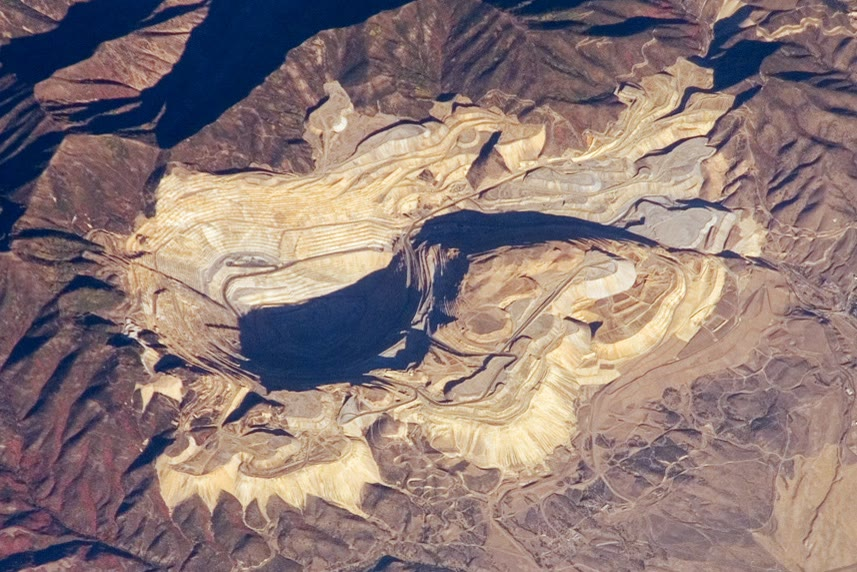
\includegraphics[width=0.5\linewidth]{images/book4/b2-29-bingham-canyon-iss.jpg}
\par\smallskip{\small De dagbouwmijn van Bingham Canyon, Utah, gezien vanuit het Internationaal Ruimtestation
(2007): meer dan \qty{4}{km} breed en \qty{1200}{m} diep, in terrassen van 16 tot \qty{25}{m} hoog
uitgegraven in een \omterm{def:b2:ore-deposits:hydrothermal}{porfierkoperafzetting}; de heuvels met vlakke top eromheen zijn afvalgesteente. Foto
NASA, Expedition 15 crew (publiek domein).}
\end{omfigure}
% ledger: photo:b2-29-bingham

\begin{definition}[Ertsafzettingstype]\label{def:b2:ore-deposits:types}
Een \emph{ertsafzettingstype}\index{ertsafzettingstype} is een klasse afzettingen met een gemeenschappelijke geologische
setting, een gastgesteente, een vorm, een ertsmineralogie en een vormingsproces, zodat een beschrijving van
de klasse voorspelt waar haar leden voorkomen. De typen vallen naar proces uiteen in vier families:
magmatisch (het metaal wordt door een \omterm{def:b2:magma-emplacement:magma}{magma} geconcentreerd terwijl het kristalliseert of ontmengt),
hydrothermaal (door een hete waterige vloeistof), sedimentair (door transport en afzetting
van sediment, of neerslag uit water aan het oppervlak) en supergeen (door verwering
van een eerdere afzetting).
\end{definition}

\section{Magmatische afzettingen}\label{sec:b2:ore-deposits:magmatic}

\textbf{Chromiet in \omterm{def:b2:magmatic-differentiation:cumulate}{gelaagde intrusies}.} Chromiet, de enige commerciële bron van chroom,
verzamelt zich in lagen massief chromitiet, meer dan \qty{90}{\percent} chromiet, in de ultramafische
onderste delen van \omterm{def:b2:magmatic-differentiation:cumulate}{gelaagde intrusies}. De intrusies zijn 2 tot \qty{180}{km} breed en tot
\qty{15}{km} dik, en de lagen variëren van minder dan een centimeter tot 5--\qty{8}{m}; samen
bevatten ze het grootste deel van de chroomreserves ter wereld, en het Bushveldcomplex, besproken in
\cref{ch:b2:magmatic-differentiation}, is de enige die vandaag op chromiet wordt ontgonnen. Hun oorsprong, een
cumulaatlaag die in het stabiliteitsveld van chromiet werd gedwongen door het mengen van \omterm{def:b2:magma-emplacement:magma}{magma's} of een verandering van druk of
oxidatietoestand, staat nog ter discussie.
% ledger: usgs10e:chromite

\textbf{Nikkel--koper--PGE-sulfiden.} Een mafisch of ultramafisch \omterm{def:b2:magma-emplacement:magma}{magma}, ontstaan bij hoge graden van
mantelsmelting (\qty{20}{\percent} tot \qty{25}{\percent} of meer, met meer dan 12 gewichtsprocent MgO),
stijgt op terwijl het onverzadigd is aan zwavel. Als het zwavel uit de korst assimileert, of ver
genoeg afkoelt, raakt het verzadigd en scheidt zich een niet-mengbare sulfidesmelt af in druppels. De
chalcofiele metalen gaan over in deze druppels: de verhouding $D$ van hun concentratie in de
sulfidesmelt tot die in de \omterm{def:b2:magma-emplacement:magma}{silicaatsmelt}, hetzelfde soort verdelingscoëfficiënt als tussen een
mineraal en een smelt, is $10^2$ tot $10^3$ voor koper en nikkel en $10^3$ tot $10^4$ voor de
platinagroepelementen. Hoeveel metaal een druppel verzamelt, hangt dan af van hoeveel \omterm{def:b2:magma-emplacement:magma}{magma} hij ontmoet.
% ledger: usgs10i:r-factor

\begin{proposition}[R-factor]\label{prop:b2:ore-deposits:r-factor}
Laat een massa-eenheid sulfidesmelt zich afscheiden uit, en in evenwicht komen met, een massa $R$
silicaatmagma, de \emph{R-factor}\index{R-factor}, in een gesloten systeem; zij $C_L$ de concentratie van een
metaal in het \omterm{def:b2:magma-emplacement:magma}{magma} voordat het sulfide zich afscheidde, en $D$ zijn verdelingscoëfficiënt tussen sulfide en silicaat.
Dan is de concentratie van het metaal in het sulfide
\begin{equation}
C_S = C_L\,\frac{D\,(R + 1)}{R + D} .
\label{eq:b2:ore-deposits:r-factor}
\end{equation}
Voor $R \gg D$ geldt $C_S \to D\,C_L$; voor $R \ll D$ geldt $C_S \approx (R + 1)\,C_L$.
\end{proposition}

\begin{proof}
Het systeem met massa $R + 1$ bevatte vóór de afscheiding $(R + 1)C_L$ van het metaal. Daarna bevat het silicaat
$R\,C_{\mathrm{sil}}$ en het sulfide $C_S$, met $C_S = D\,C_{\mathrm{sil}}$ in evenwicht.
Behoud geeft $(R + 1)C_L = R\,C_S/D + C_S = C_S\,(R + D)/D$, en daarmee
\eqref{eq:b2:ore-deposits:r-factor}. Als $R \gg D$, gaat $(R + 1)/(R + D) \to 1$; als $R \ll D$, gaat
$D/(R + D) \to 1$.
\end{proof}

De twee limieten verklaren waarom er twee soorten sulfide-erts bestaan. Wanneer $R \ll D$, neemt het sulfide
bijna al het metaal op van het \omterm{def:b2:magma-emplacement:magma}{magma} dat het ontmoet en groeit $C_S$ met $R$; wanneer $R \gg D$, is het
verzadigd bij $D\,C_L$ en voegt meer \omterm{def:b2:magma-emplacement:magma}{magma} niets toe. Nikkel en koper, met een $D$ van enkele honderden,
bereiken hun plafond bij een $R$ van enkele honderden tot enkele duizenden, het bereik van de meeste
nikkel--koperertsen; platina en palladium, met een $D$ rond $10^4$, blijven winnen tot een $R$ van \num{10000} tot
\num{100000}. Ertsen die rijk zijn aan platinagroepelementen, zoals het Merensky-rif van het Bushveld en
sommige ertsen van Norilsk, getuigen dus van een kleine massa sulfide die door een zeer grote massa
\omterm{def:b2:magma-emplacement:magma}{magma} is gespoeld (oefeningen~\ref{exo:b2:ore-deposits:5} en~\ref{exo:b2:ore-deposits:11}).
% ledger: usgs10i:r-factor

\textbf{Kimberlieten en diamanten.} De meeste diamanten, en bijna alle gewonnen exemplaren, ontstonden aan de basis van
dikke continentale lithosfeer, in de wortels van \omterm{def:b2:precambrian-earth:craton}{cratons}; kimberlietmagma's, die van diepten
groter dan 120 tot \qty{150}{km} komen en met tot \qty{20}{m.s^{-1}} opstijgen, brengen ze snel genoeg naar het
oppervlak om ze te laten overleven. Kimberlieten breken bij voorkeur door dikke, oude lithosfeer heen,
en daar zoekt de diamantexploratie.
% ledger: grabreck22:kimberlite

\textbf{Pegmatieten.} Lithium--cesium--tantaalpegmatieten zijn granitische \omterm{def:b2:magma-emplacement:bodies}{gangen} die verrijkt zijn in deze zeldzame
elementen, gevormd in collisiegebergten; ze kristalliseren bij ongeveer 350 tot \qty{550}{\celsius},
opmerkelijk laag voor een granitische smelt, in dagen tot jaren, en laten enorme kristallen groeien --- één
spodumeenkristal was \qty{14}{m} lang. Hun lithiummineralen, spodumeen, petaliet en
lepidoliet, leveren ongeveer een kwart van het lithium ter wereld.
% ledger: usgs10o:lct

\section{Hydrothermale afzettingen}\label{sec:b2:ore-deposits:hydrothermal}

\begin{definition}[Hydrothermale vloeistof en typen hydrothermale afzettingen]\label{def:b2:ore-deposits:hydrothermal}
Een \emph{hydrothermale vloeistof}\index{hydrothermale vloeistof} is een hete waterige vloeistof, vrijgekomen uit een \omterm{def:b2:magma-emplacement:magma}{magma}
of bij \omterm{def:b2:metamorphic-facies:reaction}{metamorfe reacties}, of verhit zeewater, meteorisch water of bekkenpekel, die elementen oplost,
transporteert en afzet terwijl ze door gesteente stroomt. De belangrijkste typen hydrothermale \omterm{def:b2:ore-deposits:deposit}{ertsafzettingen}
zijn:
\begin{itemize}
  \item de \emph{porfierkoperafzetting}\index{porfierkoperafzetting}: een groot lichaam met een laag gehalte
        van adertjes en verspreide kopersulfiden in en rond een kleine porfierstock, gevormd door
        magmatische vloeistoffen binnen enkele kilometers van het oppervlak boven een subductiezone;
  \item de \emph{epithermale afzetting}\index{epithermale afzetting}: goud--zilveraders en
        -verspreidingen, gevormd binnen ongeveer \qty{1.5}{km} van het oppervlak, bij ongeveer 100 tot
        \qty{300}{\celsius}, in vulkanische bogen;
  \item de \emph{vulkanogene massieve-sulfideafzetting}\index{vulkanogene massieve-sulfideafzetting}
        (VMS): een lens van massieve sulfiden gevormd op of net onder de zeebodem, bij een hydrothermale
        bron in een onderzeese vulkanische omgeving;
  \item de \emph{sedimentair-exhalatieve afzetting}\index{sedimentair-exhalatieve afzetting} (sedex):
        gelamineerde zink--loodsulfiden in mariene schalies van een \omterm{def:b2:basins-compared:types}{riftbekken}, neergeslagen op of net
        onder de zeebodem uit bekkenpekels die langs breuken opstijgen;
  \item de \emph{afzetting van het Mississippi Valley-type}\index{afzetting van het Mississippi Valley-type} (MVT):
        zink--loodsulfiden die platformcarbonaten vervangen, epigenetisch en los van
        stollingsactiviteit, afgezet door bekkenpekels;
  \item de \emph{orogene goudafzetting}\index{orogene goudafzetting}: goudhoudende kwartsaders in
        metamorfe gordels, langs grote breuken, afgezet door CO$_2$-rijke vloeistoffen met een laag zoutgehalte en van
        metamorfe oorsprong.
\end{itemize}
\end{definition}
% ledger: usgs10b:form, usgs10q:epithermal, usgs10c:vms, usgs10n:sedex, usgs10a:mvt, drew03:orogenic

\textbf{Transport en afzetting.} De meeste metalen worden in \omterm{def:b2:ore-deposits:hydrothermal}{hydrothermale vloeistoffen} als complexen vervoerd:
zink, lood en koper als chloridecomplexen, zodat het zoutgehalte hun oplosbaarheid bepaalt, en goud,
in gereduceerde vloeistoffen, als zwavelcomplexen zoals AuHS(H$_2$S)$_3$. Een vloeistof laat haar lading vallen wanneer de
oplosbaarheid daalt: wanneer ze afkoelt; wanneer ze kookt doordat haar druk daalt, waarbij ze H$_2$S en CO$_2$ verliest en
haar pH verandert; wanneer ze zich mengt met een vloeistof van andere samenstelling --- een pekel die water ontmoet dat rijk is
aan H$_2$S, slaat vrijwel meteen sfaleriet en galeniet neer; en wanneer ze reageert met het omringende
gesteente, wat haar pH of oxidatietoestand verandert. Elk afzettingstype is één combinatie van vloeistof,
pad en val.
% ledger: usgs10n:sedex, drew03:orogenic

\textbf{Porfierkoper.} Porfierafzettingen leveren ongeveer \qty{60}{\percent} van het koper ter wereld
en bevatten ongeveer \qty{65}{\percent} van de voorraden. Ze zijn gecentreerd op kleine cilindrische
stocks of gangenzwermen, de toppen van grotere \omterm{def:b2:magma-emplacement:bodies}{plutonen}, geplaatst op minder dan 5--\qty{10}{km} diepte in
bogen boven subductiezones, de omgeving van \cref{ch:b2:magmatic-series}. Een afzetting is 0.1 tot
\qty{1}{km} breed, met een vergelijkbare hoogte; omgezet gesteente kan zich \qty{10}{km} of meer eromheen uitstrekken.
Terwijl het \omterm{def:b2:magma-emplacement:magma}{magma} kristalliseert, scheidt zich een vloeistof met 3 tot 5 gewichtsprocent zout af; bij het opstijgen en
de drukverlaging splitst ze zich in een pekel en een damp, die beide metalen vervoeren, en haar overdruk
breekt het gesteente. Kwartsaders slaan neer bij ongeveer 700 tot \qty{500}{\celsius}, en de
reactie van de vloeistof met het gesteente zoneert de omzetting, zoals in de doorsnede hieronder. Omdat ze
ondiep ontstaan aan actieve randen, waar de erosie snel is, is meer dan \qty{90}{\percent} van de bekende
porfierafzettingen van cenozoïsche of mesozoïsche ouderdom.
% ledger: usgs10b:share, usgs10b:form, usgs10b:fluids, usgs10b:alteration

\begin{omfigure}
\centering
\begin{tikzpicture}[x=1.15cm, y=1.15cm, font=\small]
\begin{scope}
\clip (-2.9,-3.6) rectangle (2.9,0);
% propylitic halo
\fill[omLithBasalt!45] (0,-1.25) ellipse (2.45 and 1.55);
% sodic-calcic deep flanks
\fill[omExo!25] (-1.75,-2.55) ellipse (0.45 and 0.38);
\fill[omExo!25] (1.75,-2.55) ellipse (0.45 and 0.38);
% sericitic shell
\fill[yellow!35] (0,-1.05) ellipse (1.15 and 1.15);
% potassic core
\fill[omProp!40] (0,-1.45) ellipse (0.68 and 0.85);
% ore shell
\draw[omThm, line width=1.1pt, densely dashed] (0,-1.3) ellipse (0.92 and 0.98);
% advanced argillic lithocap
\fill[omDef!30] (-1.05,0) .. controls (-0.6,-0.5) and (0.6,-0.5) .. (1.05,0) -- cycle;
\draw[omDef!70] (-1.05,0) .. controls (-0.6,-0.5) and (0.6,-0.5) .. (1.05,0);
\end{scope}
% pluton and stock
\fill[omLithGranite] (-2.6,-3.6) .. controls (-2.2,-2.9) and (-0.9,-2.6) .. (-0.3,-2.6)
  -- (-0.3,-1.25) arc[start angle=180, end angle=0, radius=0.3] -- (0.3,-2.6)
  .. controls (0.9,-2.6) and (2.2,-2.9) .. (2.6,-3.6) -- cycle;
\draw[black!60] (-2.6,-3.6) .. controls (-2.2,-2.9) and (-0.9,-2.6) .. (-0.3,-2.6)
  -- (-0.3,-1.25) arc[start angle=180, end angle=0, radius=0.3] -- (0.3,-2.6)
  .. controls (0.9,-2.6) and (2.2,-2.9) .. (2.6,-3.6);
% epithermal veins
\foreach \x in {1.45,1.65,1.85} \draw[omDef, line width=1pt] (\x,-0.02) -- (\x+0.12,-0.7);
% palaeosurface
\draw[black, line width=0.8pt] (-2.9,0) -- (2.9,0);
\node[anchor=south west, font=\scriptsize] at (-2.9,0) {paleo-oppervlak};
% labels
\draw[black!50] (0.6,-0.15) -- (1.2,0.25) -- (3.0,0.25) node[anchor=west, text=black] {geavanceerd argillisch};
\draw[black!50] (1.95,-0.3) -- (3.0,-0.3) node[anchor=west, text=black] {epithermale aders};
\draw[black!50] (1.05,-0.8) -- (3.0,-0.8) node[anchor=west, text=black] {sericitisch};
\draw[black!50] (0.85,-1.25) -- (3.0,-1.25) node[anchor=west, text=omThm] {ertsschil van koper};
\draw[black!50] (0.45,-1.7) -- (3.0,-1.7) node[anchor=west, text=black] {potassisch};
\draw[black!50] (1.05,-2.15) -- (3.0,-2.15) node[anchor=west, text=black] {propylitisch};
\draw[black!50] (2.1,-2.6) -- (3.0,-2.6) node[anchor=west, text=black] {natrium--calcium};
\draw[black!50] (1.5,-3.15) -- (3.0,-3.15) node[anchor=west, text=black] {pluton en porfierstock};
\end{tikzpicture}
\par\smallskip{\small Een porfierkopersysteem in doorsnede (een tekening, niet op schaal): de potassische
zone in de kern, diep en heet; de sericitische zone naar boven en naar buiten, waar pyriet
overvloedig is; de ertsschil van koper ertussen; de propylitische halo op geringe tot middelgrote diepte
eromheen; natrium--calciumomzetting op de diepe flanken; een geavanceerd argillische kap en, in sommige
systemen, epithermale aders dicht bij het oppervlak.}
\end{omfigure}
% ledger: usgs10b:alteration

\textbf{Epithermaal goud.} Boven sommige porfiersystemen, en in vulkanische bogen in het algemeen, bereiken
dezelfde soort vloeistoffen de bovenste \qty{1.5}{km} van de korst bij ongeveer 100 tot \qty{300}{\celsius},
waar ze koken en zich mengen met grondwater; ze zetten goud en zilver af in kwartsaders, met een
omzetting die bijna neutrale vloeistoffen (adularia, illiet) of zeer zure (kaoliniet,
dickiet, pyrofylliet) vastlegt.
% ledger: usgs10q:epithermal, usgs10q:alteration

\textbf{Massieve sulfiden op de zeebodem.} Zeewater dat in de hete korst van een rug of
een boog wordt gezogen, keert bij bronnen terug als zwarte rokers van ongeveer \qty{350}{\celsius}, voor het eerst gezien op de
Oost-Pacifische Rug in 1979. Waar het bronnenveld lang genoeg bestaat, bouwen de sulfiden ervan een heuvel op; het erts bestaat voor meer dan
\qty{40}{\percent} uit sulfiden, boven een stockwork van aders dat de toevoer markeert. De metalen zijn gezoneerd
naar temperatuur, ijzer en koper aan de hete basis, zink, ijzer, lood en barium aan de koelere top en
randen, zoals in de heuvel die in de volgende paragraaf is getekend. \omterm{def:b2:ore-deposits:hydrothermal}{Vulkanogene
massieve-sulfideafzettingen} variëren van lenzen van minder dan een ton tot de \qty{1.5}{Gt} van Rio Tinto in Spanje, en in
ouderdom van \qty{3.55}{\Ga} tot afzettingen die zich vandaag vormen.
% ledger: usgs10c:vms

\textbf{Bekkenpekels: sedex en MVT.} Bekkenpekels met 10 tot \qty{30}{\percent} opgeloste zouten,
door begraving verhit tot 100--\qty{200}{\celsius}, vervoeren zink en lood als chloridecomplexen en vormen de
twee typen in sedimentair gastgesteente. Sedex-afzettingen ontstaan waar de pekel langs een riftbreuk uittreedt in een afgesloten, gereduceerd
bekken en waterstofsulfide ontmoet, wat gelamineerde sulfidemodder oplevert; ze bevatten meer
dan de helft van de zink- en loodreserves ter wereld. MVT-afzettingen ontstaan waar de pekel, uit een
bekken verdreven, aan de rand ervan een carbonaatplatform bereikt en het vervangt bij 75 tot ongeveer
\qty{200}{\celsius}; ze bevatten \qty{38}{\percent} van het lood en zink van de afzettingen in sedimentair gastgesteente,
met ongeveer tien keer meer zink dan lood.
% ledger: usgs10n:sedex, usgs10a:mvt

\textbf{Orogeen goud.} In metamorfe gordels maken ontgassingsreacties een bijna neutrale vloeistof
met een laag zoutgehalte en rijk aan CO$_2$ vrij; langs grote breuken gekanaliseerd, zet ze goudhoudende
kwartsaders af bij ongeveer \qty{350}{\celsius} en 4 tot \qty{12}{km} diepte. De aders lopen door over
grote hoogten: \qty{3.2}{km} in Kolar, in India.
% ledger: drew03:orogenic

\section{Sedimentaire en supergene afzettingen}\label{sec:b2:ore-deposits:sedimentary}

\begin{definition}[Placer]\label{def:b2:ore-deposits:placer}
Een \emph{placer}\index{placer} is een sedimentaire afzetting van dichte, duurzame mineralen die geconcentreerd zijn door
stromend water of wind omdat ze, bij dezelfde grootte, sneller bezinken en minder gemakkelijk worden meegevoerd
dan de kwartskorrels eromheen.
\end{definition}

Mineralen met een dichtheid boven ongeveer 2.85 heten zwaar, tegenover 2.65 voor kwarts: ilmeniet en zirkoon
rond 4.7, magnetiet 5.2, goud 15 tot 19.3. Volgens de wet van Stokes groeit de bezinkingssnelheid van een korrel met
zijn dichtheidsoverschot $\rho_s - \rho_w$, elf keer groter voor goud dan voor kwarts, zodat goud van een
gegeven grootte samen ligt met kwarts van driemaal die grootte (oefening~\ref{exo:b2:ore-deposits:3}); goud
blijft meestal in riviergrind op het vaste gesteente, terwijl ilmeniet, rutiel en zirkoon stranden en
duinen bereiken. Gehalten in zwaremineralenzanden zijn het gewichtspercentage zware mineralen.
% ledger: usgs10l:heavy, usgs:gold-placer

Chemische sedimenten zijn ook ertsen. De \omterm{def:b2:precambrian-earth:bif}{gebande ijzerformaties} van \cref{ch:b2:precambrian-earth},
neergeslagen toen het opgeloste ijzer van de oceanen werd geoxideerd, zijn een gewoon ijzererts; evaporieten
leveren haliet en de kaliumzouten; laterieten, het residu van diepe tropische verwering,
concentreren aluminium als bauxiet. Verwering verrijkt ook eerdere afzettingen.
% ledger: earle:bif, usgs:bauxite

\begin{definition}[Supergene verrijking, ijzeren hoed]\label{def:b2:ore-deposits:supergene}
\emph{Supergene verrijking}\index{supergene verrijking} is de concentratie van een metaal door
dalend grondwater: boven de grondwaterspiegel lost zuurstofrijk, zuur water het metaal op uit de
sulfiden van een ertslichaam, en daaronder, in reducerende omstandigheden, zet het dat weer af, meestal door
de primaire sulfiden te vervangen. Een \emph{ijzeren hoed}\index{ijzeren hoed} (gossan) is het poreuze, ijzeroxiderijke gesteente
dat aan het oppervlak achterblijft boven een verweerd sulfidelichaam, waarvan de sulfiden zijn vervangen door goethiet, hematiet en
jarosiet.
\end{definition}

In porfierafzettingen is de uitgeloogde kap boven de grondwaterspiegel tot enkele honderden meters
dik; daaronder bereiken verrijkte sulfidezones van chalcosien, tientallen tot enkele honderden meters dik,
meer dan \qty{1.5}{Gt} met 0.4 tot \qty{1.7}{\percent} koper, altijd rijker dan het primaire,
hypogene erts eronder. De ijzeroxiden van een \omterm{def:b2:ore-deposits:supergene}{ijzeren hoed} en van een uitgeloogde kap behouden de texturen van de
sulfiden die ze vervingen, en wijzen de weg bij het zoeken eronder; \omterm{def:b2:ore-deposits:supergene}{ijzeren hoeden} en hun ijzervlekken onthulden aan vroege mijnwerkers veel
afzettingen van massieve sulfiden.
% ledger: usgs10b:supergene, usgs10c:vms

\begin{omfigure}
\centering
\begin{minipage}[b]{0.46\linewidth}\centering
\begin{tikzpicture}[x=1cm, y=1cm, font=\scriptsize]
\fill[omHist!55] (0,4.0) rectangle (1.8,5.2);
\fill[omMeth!30] (0,3.0) rectangle (1.8,4.0);
\fill[black!55] (0,1.8) rectangle (1.8,3.0);
\fill[black!18] (0,0) rectangle (1.8,1.8);
\draw (0,0) rectangle (1.8,5.2);
\draw[omDef, line width=1pt, densely dashed] (-0.25,3.0) -- (2.05,3.0);
\foreach \x in {0.45,0.9,1.35} \draw[omDef, -{Stealth[length=4pt]}] (\x,5.0) -- (\x,3.2);
\node[anchor=west, align=left] at (2.0,4.6) {ijzeren hoed en\\uitgeloogde kap\\(Fe-oxiden)};
\node[anchor=west, align=left] at (2.0,3.5) {oxidezone\\(malachiet)};
\node[anchor=east, text=omDef, align=right] at (-0.25,3.0) {grondwater-\\spiegel};
\node[anchor=west, align=left] at (2.0,2.4) {verrijkingsdeken\\(chalcosien)};
\node[anchor=west, align=left] at (2.0,0.9) {primair erts\\(chalcopyriet\\+ pyriet)};
\node[anchor=south, font=\scriptsize, text=omDef] at (0.9,5.25) {zuur water, Cu$^{2+}$};
\end{tikzpicture}
\end{minipage}\hfill
\begin{minipage}[b]{0.52\linewidth}\centering
\begin{tikzpicture}[x=1cm, y=1cm, font=\scriptsize]
\fill[omSea] (-2.6,1.4) rectangle (2.6,3.2);
\fill[omLithBasalt!60] (-2.6,-1.6) rectangle (2.6,1.4);
% stockwork cone
\fill[omProp!25] (-0.5,-1.6) -- (0.5,-1.6) -- (1.1,0.9) -- (-1.1,0.9) -- cycle;
\foreach \x/\y in {-0.3/-1.2,0.1/-1.0,-0.6/-0.4,0.4/-0.3,-0.1/0.1,0.6/0.4,-0.7/0.5}
  \draw[omProp!80!black] (\x,\y) -- ++(0.35,0.25);
% mound: upper rim and core
\fill[yellow!45] (-1.8,1.4) .. controls (-1.2,2.35) and (1.2,2.35) .. (1.8,1.4) -- cycle;
\fill[omThm!45] (-1.1,1.4) .. controls (-0.7,2.0) and (0.7,2.0) .. (1.1,1.4) -- cycle;
\draw (-1.8,1.4) .. controls (-1.2,2.35) and (1.2,2.35) .. (1.8,1.4);
% chimney and plume
\fill[black!70] (-0.08,2.1) rectangle (0.08,2.55);
\fill[black!45] (0,2.6) circle (0.12) (0.1,2.8) circle (0.16) (0.25,3.0) circle (0.2);
\draw[omDef, -{Stealth[length=4pt]}] (-2.3,2.9) -- (-2.3,0.2) -- (-1.2,-0.9);
\draw[omThm, -{Stealth[length=4pt]}] (0,-1.5) -- (0,1.2);
\node[anchor=west, text=omDef] at (-2.55,3.05) {zeewater};
\node[anchor=west] at (0.45,2.85) {zwarte roker, \qty{350}{\celsius}};
\draw[black!50] (1.45,1.75) -- (2.0,2.15) node[anchor=west, text=black] {Zn, Fe, Pb, Ba};
\draw[black!50] (0.6,1.6) -- (2.0,1.15) node[anchor=west, text=black] {Fe, Cu};
\node[anchor=west, align=left] at (0.95,-0.4) {stockwork\\(toevoer)};
\node[anchor=north, text=omThm] at (0,-1.6) {hete vloeistof};
\end{tikzpicture}
\end{minipage}
\par\smallskip{\small Links: een supergeen profiel boven een kopersulfidelichaam (een tekening, niet op
schaal): zuur water loogt koper uit boven de grondwaterspiegel en zet het daaronder weer af als chalcosien,
met een \omterm{def:b2:ore-deposits:supergene}{ijzeren hoed} aan het oppervlak als restant. Rechts: een vulkanogene massieve-sulfideheuvel in doorsnede (een
tekening): zeewater dat in de korst wordt verhit, stijgt op door een stockwork en treedt uit als een zwarte roker; de
heuvel is gezoneerd van ijzer en koper aan de hete basis tot zink, ijzer, lood en barium aan de top en de
randen.}
\end{omfigure}
% ledger: usgs10b:supergene, usgs10c:vms

\begin{omfigure}
\centering
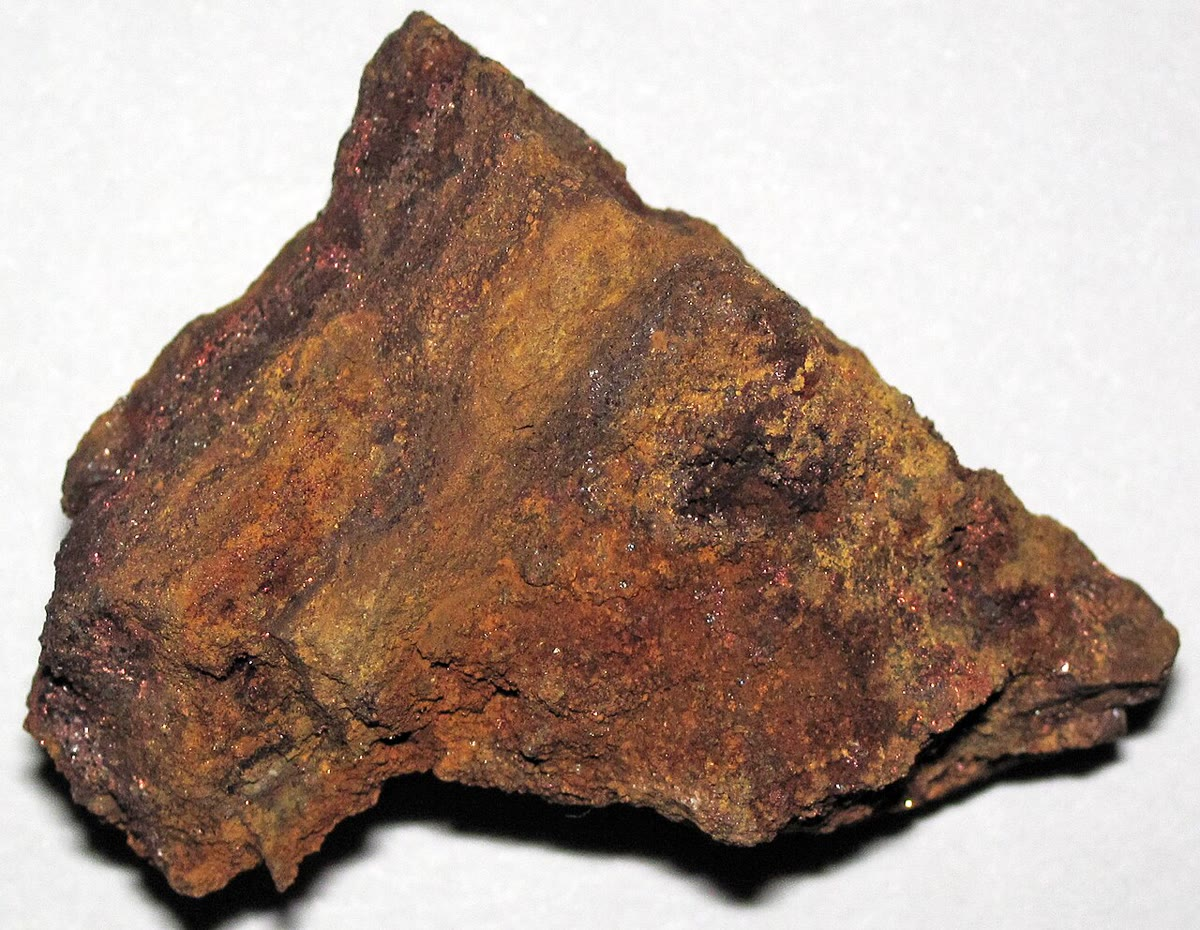
\includegraphics[width=0.4\linewidth]{images/book4/b2-29-flambeau-gossan.jpg}
\par\smallskip{\small IJzeren hoed van de massieve-sulfideafzetting van Flambeau, Wisconsin: een poreus gesteente van
ijzerhydroxy-oxiden, achtergebleven na de verwering van pyriet, chalcopyriet, chalcosien en borniet in een
paleoproterozoïsche vulkanische boog; de kleine oranje vlekjes zijn gedegen koper. Foto James St.
John (CC BY 2.0).}
\end{omfigure}
% ledger: photo:b2-29-gossan

\section{Gehalte en tonnage}\label{sec:b2:ore-deposits:grade-tonnage}

Een wereldwijde compilatie vermeldt 422 \omterm{def:b2:ore-deposits:hydrothermal}{porfierkoperafzettingen} met hun \omterm{def:b2:ore-deposits:grade}{tonnage}, bij het laagste beschikbare
\omterm{def:b2:ore-deposits:grade}{grensgehalte}, en hun gemiddelde kopergehalte. Een tiende ervan overschrijdt \qty{1500}{Mt} en een tiende bevat minder
dan \qty{33}{Mt}, met een mediaan van \qty{240}{Mt}; de gehalten lopen van \qty{0.24}{\percent} tot
\qty{0.75}{\percent} tussen dezelfde decielen, met een mediaan van \qty{0.44}{\percent}. Tussen de
decielen spreidt de \omterm{def:b2:ore-deposits:grade}{tonnage} zich over een factor 45, het gehalte over een factor 3. Op logaritmische assen liggen beide histogrammen dicht bij normale curven, zoals de figuur hieronder toont:
de logaritmen van de \omterm{def:b2:ore-deposits:grade}{tonnage} hebben een gemiddelde van 2.373 en een standaardafwijking van 0.654, die van het gehalte
$-0.364$ en 0.199 (logaritmen met grondtal 10, \omterm{def:b2:ore-deposits:grade}{tonnage} in megaton, gehalte in procent). De aanpassing is
onvolmaakt: de gehalten zijn spitser verdeeld dan een lognormale wet, en enkele afzettingen met een zeer laag gehalte doen
ze in een formele toets ervan afwijken. En de twee zijn bijna onafhankelijk, met een correlatie van
0.1 tussen hun logaritmen.
% ledger: usgs08:table1, usgs08:independence, data:b4-porphyry-cu

\begin{omfigure}
\centering
\begin{minipage}[b]{0.49\linewidth}\centering
\begin{tikzpicture}
\begin{axis}[omrecord, width=0.96\linewidth, height=4.5cm, xmin=0.5, xmax=5.0, ymin=0, ymax=80,
  xlabel={tonnage (Mt)}, ylabel={aantal afzettingen},
  xtick={1,2,3,4,5}, xticklabels={10,100,1000,$10^4$,$10^5$},
  tick label style={font=\scriptsize}, label style={font=\small}]
% computed in figdata/bachelor-2/ores.py part hist_t; ledger: data:b4-porphyry-cu
\addplot[ybar, bar width=0.22, fill=omDef!35, draw=omDef!70] table[x=log10_t, y=count] {figdata/out/bachelor-2-ores-hist_t.dat};
\addplot[omThm, line width=1pt, smooth] table[x=log10_t, y=fit] {figdata/out/bachelor-2-ores-hist_t.dat};
\end{axis}
\end{tikzpicture}
\end{minipage}\hfill
\begin{minipage}[b]{0.49\linewidth}\centering
\begin{tikzpicture}
\begin{axis}[omrecord, width=0.96\linewidth, height=4.5cm, xmin=-1.2, xmax=0.6, ymin=0, ymax=120,
  xlabel={kopergehalte (\%)}, ylabel={aantal afzettingen},
  xtick={-1,-0.69897,-0.30103,0,0.30103}, xticklabels={0.1,0.2,0.5,1,2},
  tick label style={font=\scriptsize}, label style={font=\small}]
% computed in figdata/bachelor-2/ores.py part hist_g; ledger: data:b4-porphyry-cu
\addplot[ybar, bar width=0.088, fill=omDef!35, draw=omDef!70] table[x=log10_g, y=count] {figdata/out/bachelor-2-ores-hist_g.dat};
\addplot[omThm, line width=1pt, smooth] table[x=log10_g, y=fit] {figdata/out/bachelor-2-ores-hist_g.dat};
\end{axis}
\end{tikzpicture}
\end{minipage}
\par\smallskip{\small De \omterm{def:b2:ore-deposits:grade}{tonnage} (links) en het kopergehalte (rechts) van de 422
\omterm{def:b2:ore-deposits:hydrothermal}{porfierkoperafzettingen} van de wereldwijde compilatie, op logaritmische assen, met in rood de normale curven met hetzelfde gemiddelde
en dezelfde standaardafwijking. Gegevens: Singer, Berger en Moring (2008), USGS.}
\end{omfigure}

\begin{proposition}[Product van lognormale variabelen]\label{prop:b2:ore-deposits:product}
Als $\log_{10} T$ en $\log_{10} g$ gezamenlijk normaal verdeeld zijn, met gemiddelden $\mu_T$ en $\mu_g$,
standaardafwijkingen $\sigma_T$ en $\sigma_g$ en correlatie $\rho$, dan is de metaalinhoud $M = Tg/100$
($g$ in procent) lognormaal: $\log_{10} M$ is normaal verdeeld met
\begin{equation}
\mu_M = \mu_T + \mu_g - 2 , \qquad
\sigma_M^2 = \sigma_T^2 + \sigma_g^2 + 2\rho\,\sigma_T\sigma_g .
\label{eq:b2:ore-deposits:product}
\end{equation}
\end{proposition}

\begin{proof}
$\log_{10} M = \log_{10} T + \log_{10} g - 2$. Een lineaire combinatie van gezamenlijk normale variabelen is
normaal (aangenomen uit de wiskundeboeken); haar gemiddelde is de som van de gemiddelden en haar variantie
$\operatorname{var}(X + Y) = \operatorname{var} X + \operatorname{var} Y + 2\operatorname{cov}(X, Y)$,
met $\operatorname{cov}(X, Y) = \rho\,\sigma_T\sigma_g$.
\end{proof}

Voor de porfierafzettingen is $\sigma_M = \sqrt{0.654^2 + 0.199^2 + 2 \times 0.1 \times 0.654 \times
0.199} = 0.702$ en $\mu_M = 0.009$: de mediane afzetting bevat ongeveer \qty{1}{Mt} koper, en de
metaalinhoud spreidt zich nog wijder dan de \omterm{def:b2:ore-deposits:grade}{tonnage}. Een lognormale wet met zo'n grote spreiding
legt het meeste metaal in enkele afzettingen: het grootste tiende bevat volgens de wet ongeveer \qty{63}{\percent} van het
koper, \qty{64}{\percent} in de gegevens (oefening~\ref{exo:b2:ore-deposits:12}). De
figuur hieronder zet elke afzetting uit naar \omterm{def:b2:ore-deposits:grade}{tonnage} en gehalte, met lijnen van gelijke koperinhoud;
Bingham, met \qty{28.5}{Mt}, ligt tussen de lijnen van 10 en \qty{100}{Mt}.
% ledger: data:b4-porphyry-cu
% values: sd_log10_m 0.702233, mean 0.00857; median M 1.02 Mt; top 10 % share 0.631 (fit) 0.643 (data)

\begin{definition}[Gehalte--tonnagecurve]\label{def:b2:ore-deposits:gt}
De \emph{gehalte--tonnagecurve}\index{gehalte--tonnagecurve} van een afzetting geeft, als functies van
het \omterm{def:b2:ore-deposits:grade}{grensgehalte} $c$, de \omterm{def:b2:ore-deposits:grade}{tonnage} $T(c)$ van de blokken met een gehalte boven $c$ en hun gemiddelde gehalte
$\bar g(c)$.
\end{definition}

\begin{proposition}[Gehalte--tonnagecurve van een lognormale afzetting]\label{prop:b2:ore-deposits:gt}
Als de gehalten van de blokken van een afzetting met totale \omterm{def:b2:ore-deposits:grade}{tonnage} $T_0$ lognormaal zijn, met $\ln g$ normaal
met gemiddelde $\mu$ (het mediane gehalte is $e^{\mu}$) en standaardafwijking $s$, dan geldt, met $z = (\mu -
\ln c)/s$,
\begin{equation}
T(c) = T_0\,\Phi(z), \qquad
\bar g(c) = e^{\mu + s^2/2}\,\frac{\Phi(z + s)}{\Phi(z)} ,
\label{eq:b2:ore-deposits:gt}
\end{equation}
en het metaal boven het \omterm{def:b2:ore-deposits:grade}{grensgehalte} is $M(c) = T_0\,e^{\mu + s^2/2}\,\Phi(z + s)$, een fractie $\Phi(z +
s)$ van het geheel.
\end{proposition}

\begin{proof}
Schrijf $\ln g = \mu + s u$, met $u$ standaardnormaal. Een blok ligt boven het \omterm{def:b2:ore-deposits:grade}{grensgehalte} wanneer $u > (\ln c -
\mu)/s = -z$, wat kans $1 - \Phi(-z) = \Phi(z)$ heeft; vandaar $T(c)$. Het metaal boven het
\omterm{def:b2:ore-deposits:grade}{grensgehalte} per eenheid totale \omterm{def:b2:ore-deposits:grade}{tonnage} is $\int_{-z}^{\infty} e^{\mu + s u}\,\varphi(u)\,\mathrm{d}u$,
met $\varphi$ de standaardnormale dichtheid. Kwadraatafsplitsing geeft $e^{su}\varphi(u) =
e^{s^2/2}\varphi(u - s)$, zodat de integraal gelijk is aan $e^{\mu + s^2/2}\,[1 - \Phi(-z - s)] = e^{\mu +
s^2/2}\,\Phi(z + s)$. Delen door $\Phi(z)$ geeft het gemiddelde gehalte.
\end{proof}

Voor $c \to 0$ wordt de hele afzetting behouden, met het gemiddelde gehalte $e^{\mu + s^2/2}$, dat boven de
mediaan ligt. Het \omterm{def:b2:ore-deposits:grade}{grensgehalte} verhogen neemt sneller \omterm{def:b2:ore-deposits:grade}{tonnage} weg dan metaal, omdat de verwijderde blokken de
armste zijn: in de illustratieve afzetting van de figuur behoudt een verhoging van het \omterm{def:b2:ore-deposits:grade}{grensgehalte} van 0.2 tot
\qty{0.5}{\percent} \qty{41}{\percent} van de \omterm{def:b2:ore-deposits:grade}{tonnage} maar \qty{61}{\percent} van het koper.
% values: demo T 876.0/355.0 Mt, M 4.599/2.826 Mt (figdata ores.py gtcurve)

\begin{omfigure}
\centering
\begin{minipage}[b]{0.49\linewidth}\centering
\begin{tikzpicture}
\begin{axis}[omrecord, width=0.96\linewidth, height=5.0cm, xmode=log, ymode=log,
  xmin=2, xmax=50000, ymin=0.05, ymax=2.8, xlabel={tonnage (Mt)}, ylabel={kopergehalte (\%)},
  ytick={0.1,0.2,0.5,1,2}, yticklabels={0.1,0.2,0.5,1,2},
  tick label style={font=\scriptsize}, label style={font=\small}]
% computed in figdata/bachelor-2/ores.py parts scatter and iso; ledger: data:b4-porphyry-cu
\addplot[black!45, line width=0.6pt, unbounded coords=jump] table[x=tonnage_mt, y=g01] {figdata/out/bachelor-2-ores-iso.dat};
\addplot[black!45, line width=0.6pt, unbounded coords=jump] table[x=tonnage_mt, y=g1] {figdata/out/bachelor-2-ores-iso.dat};
\addplot[black!45, line width=0.6pt, unbounded coords=jump] table[x=tonnage_mt, y=g10] {figdata/out/bachelor-2-ores-iso.dat};
\addplot[black!45, line width=0.6pt, unbounded coords=jump] table[x=tonnage_mt, y=g100] {figdata/out/bachelor-2-ores-iso.dat};
\addplot[omDef, only marks, mark=*, mark size=0.8pt, opacity=0.7] table[x=tonnage_mt, y=cu_pct] {figdata/out/bachelor-2-ores-scatter.dat};
\addplot[omThm, only marks, mark=square*, mark size=2pt] coordinates {(3230,0.882)};
\node[font=\tiny, text=black!70, fill=white, inner sep=1pt] at (axis cs:4.55,2.2) {0.1};
\node[font=\tiny, text=black!70, fill=white, inner sep=1pt] at (axis cs:45.5,2.2) {1};
\node[font=\tiny, text=black!70, fill=white, inner sep=1pt] at (axis cs:455,2.2) {10};
\node[font=\tiny, text=black!70, fill=white, inner sep=1pt] at (axis cs:4545,2.2) {100 Mt};
\node[font=\scriptsize, text=omThm, anchor=south, fill=white, inner sep=1pt] at (axis cs:3230,1.0) {Bingham};
\end{axis}
\end{tikzpicture}
\end{minipage}\hfill
\begin{minipage}[b]{0.49\linewidth}\centering
\begin{tikzpicture}
\begin{axis}[omrecord, width=0.80\linewidth, height=5.0cm, xmin=0, xmax=1.2, ymin=0, ymax=1000,
  xlabel={grensgehalte (\%)}, ylabel={tonnage erboven (Mt)}, axis y line*=left,
  ylabel style={text=omDef}, tick label style={font=\scriptsize}, label style={font=\small}]
% computed in figdata/bachelor-2/ores.py part gtcurve (illustrative deposit)
\addplot[omDef, line width=1.1pt] table[x=cutoff_pct, y=tonnage_mt] {figdata/out/bachelor-2-ores-gtcurve.dat};
\end{axis}
\begin{axis}[width=0.80\linewidth, height=5.0cm, xmin=0, xmax=1.2, ymin=0, ymax=1.6,
  axis y line*=right, axis x line=none, ylabel={gemiddeld gehalte erboven (\%)},
  ylabel style={text=omThm}, tick label style={font=\scriptsize}, label style={font=\small}]
\addplot[omThm, line width=1.1pt, densely dashed] table[x=cutoff_pct, y=grade_pct] {figdata/out/bachelor-2-ores-gtcurve.dat};
\end{axis}
\end{tikzpicture}
\end{minipage}
\par\smallskip{\small Links: \omterm{def:b2:ore-deposits:grade}{tonnage} en kopergehalte van de 422 \omterm{def:b2:ore-deposits:hydrothermal}{porfierkoperafzettingen}, met
lijnen van gelijke koperinhoud (0.1 tot \qty{100}{Mt}); het rode vierkant is Bingham Canyon. Gegevens:
Singer, Berger en Moring (2008), USGS. Rechts: de \omterm{def:b2:ore-deposits:gt}{gehalte--tonnagecurve} van een illustratieve afzetting
van \qty{1000}{Mt}, mediaan gehalte \qty{0.40}{\percent}, $s = 0.60$: \omterm{def:b2:ore-deposits:grade}{tonnage} boven het \omterm{def:b2:ore-deposits:grade}{grensgehalte} (blauw)
en het gemiddelde gehalte ervan (rood, gestreept), volgens \eqref{eq:b2:ore-deposits:gt}.}
\end{omfigure}

\section{Exploratie}\label{sec:b2:ore-deposits:exploration}

Afzettingen worden gevonden aan de sporen die ze buiten hun erts nalaten. De omzettingshalo van een
porfiersysteem is kilometers breed, en waar het gesteente dagzoomt, kunnen de mineralen ervan vanuit vliegtuigen
en satellieten in kaart worden gebracht aan hun infraroodspectra; de metalen ervan verspreiden zich in de bodems, beeksedimenten, wateren en planten
eromheen; en de sulfiden en omgezette gesteenten veranderen de fysische eigenschappen die de geofysica meet.
% ledger: usgs10b:form, usgs10b:exploration, usgs10b:remote

\begin{definition}[Geochemische anomalie]\label{def:b2:ore-deposits:exploration}
Een \emph{geochemische anomalie}\index{geochemische anomalie} is een concentratie van een element, of van een
groep elementen, in een bemonsterd medium --- gesteente, bodem, beeksediment, water, planten --- die
afwijkt van de achtergrond in het gebied, het bereik van concentraties dat wordt gevonden waar geen
mineralisatie aanwezig is.
\end{definition}

Net als gehalten spreiden concentraties zich over ordes van grootte, zodat een anomalie gewoonlijk op
logaritmen wordt beoordeeld; een eenvoudige drempel, gebruikt in oefening~\ref{exo:b2:ore-deposits:9}, is het gemiddelde van
de logaritmen van de achtergrond plus tweemaal hun standaardafwijking. Een monster beeksediment
mengt het sediment van zijn hele stroomgebied, zodat een anomalie stroomafwaarts vervaagt naarmate schoon sediment
erbij komt, en de gradiënt van de concentraties wijst stroomopwaarts naar de bron. In bodems boven
begraven pegmatieten zijn anomalieën van lithium, rubidium, cesium, tantaal en tin gevolgd boven
lichamen die niet dagzomen.
% ledger: usgs10b:exploration, usgs10o:lct

Geofysische methoden worden gekozen naar het contrast dat een afzettingstype biedt. Verspreide sulfiden doen een
gesteente zich als een condensator gedragen: de methode van de geïnduceerde polarisatie, die deze oplaadbaarheid meet, werd
ontwikkeld voor porfierkoper en reageert het sterkst op de pyrietrijke sericitische zone, omdat de potassische
kern armer is aan sulfiden. Magnetische en zwaartekrachtmetingen brengen de \omterm{def:b2:magma-emplacement:bodies}{plutonen} in kaart waarmee de afzettingen
samenhangen. Geen enkele methode ziet erts
rechtstreeks, en elke interpretatie is niet eenduidig tot een boorgat haar toetst.
% ledger: usgs10b:exploration

\begin{method}[Van analyses naar een schatting van de voorraad]\label{met:b2:ore-deposits:resource}
De gegevens zijn boorgaten in een raster over de afzetting, waarvan de kern per interval van
bekende lengte is beschreven en geanalyseerd.
\begin{enumerate}
  \item \textbf{Samenstellen.} Middel de analyses over gelijke lengten, waarbij elke analyse naar haar
        lengte wordt gewogen, zodat elk samengesteld monster hetzelfde volume vertegenwoordigt.
  \item \textbf{Modelleren.} Verdeel de afzetting in blokken en schat het gehalte van elk uit de
        nabije samengestelde monsters, gewogen naar afstand en naar de ruimtelijke correlatie van de gehalten
        (de geostatistische methode van kriging, aangenomen).
  \item \textbf{Rapporteren.} Pas een \omterm{def:b2:ore-deposits:grade}{grensgehalte} toe: \omterm{def:b2:ore-deposits:grade}{tonnage} en gemiddeld gehalte van de blokken erboven, met de
        dichtheid van het gesteente, op elk betrouwbaarheidsniveau dat de boorafstand toelaat.
\end{enumerate}
\end{method}

\begin{inthefield}[Boorkernen beschrijven]
\centering
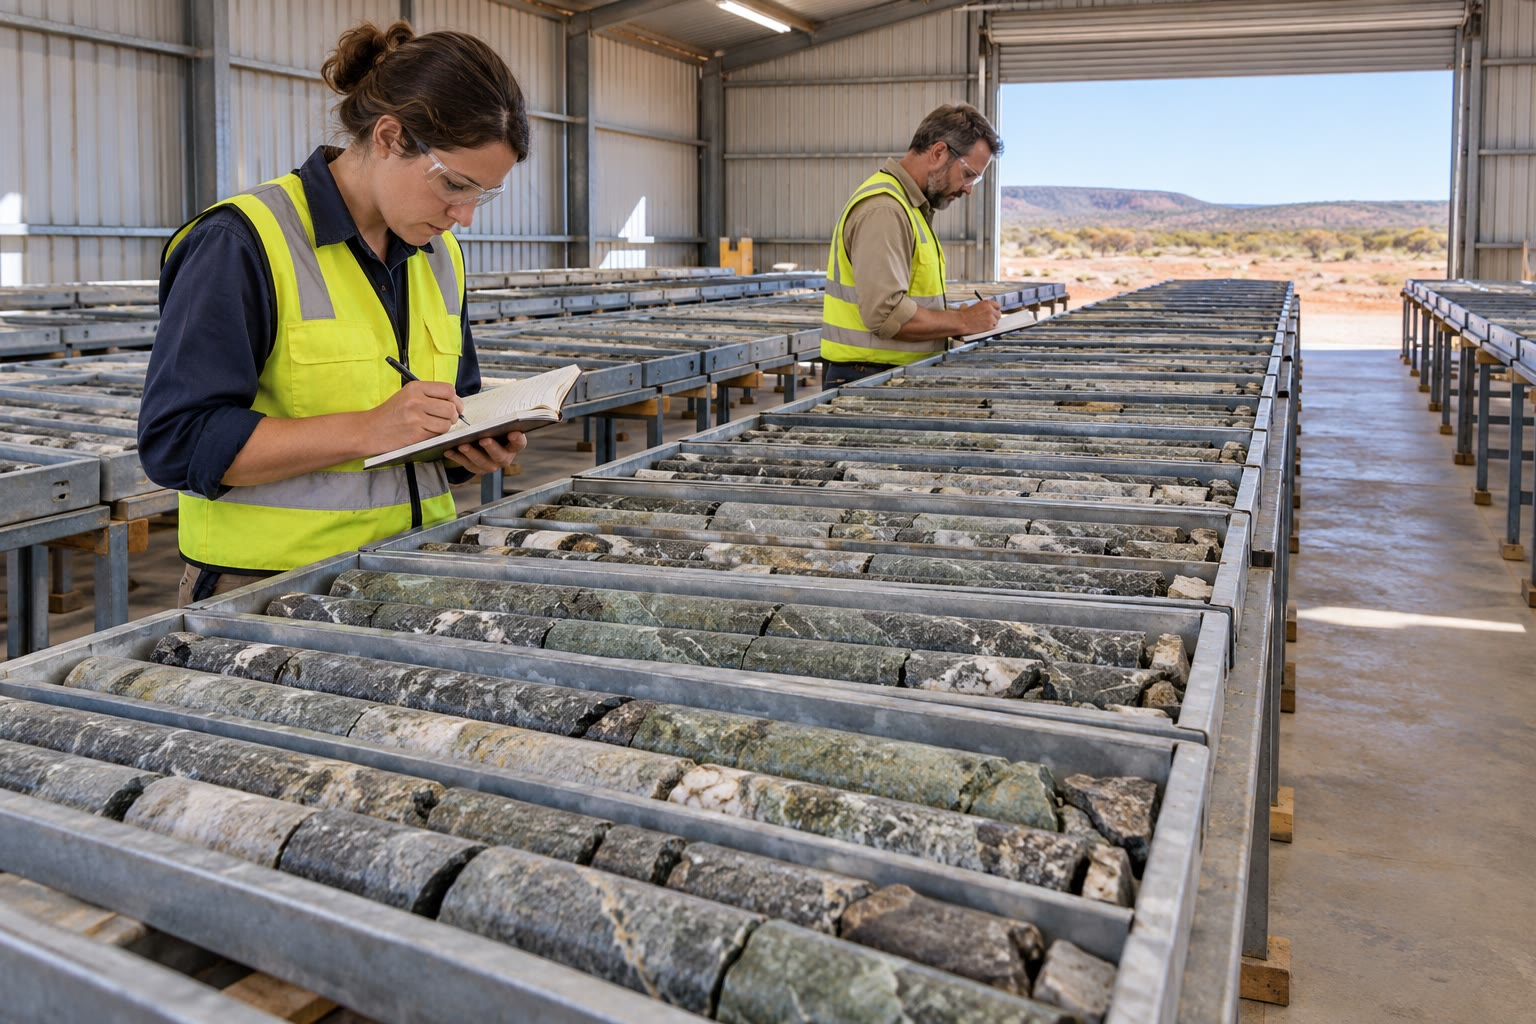
\includegraphics[width=0.56\linewidth]{images/book4/ai/b2-core-shed.jpg}
\par\smallskip{\small Een kernloods bij een exploratieproject (door AI gegenereerde illustratie).}
\par\medskip\raggedright
Bij een exploratieproject wordt de kern van elk boorgat uitgelegd in metalen bakken, in de volgorde
waarin hij uit de grond kwam. Geologen lopen de bakken af, interval na interval, en noteren wat het
gesteente is, hoe het is omgezet, welke aders het doorsnijden en in welke verhouding, en welke sulfiden het
bevat; ze markeren waar de kern zal worden gezaagd en bemonsterd. De beschrijving gaat aan de analyses vooraf en wordt
ermee vergeleken: een omzettingszone of een adertype dat het metaal draagt, wordt het spoor dat
van gat tot gat wordt gevolgd, en uit de beschrijving tekenen de geologen de doorsneden waarop de volgende
gaten worden gepland.
\end{inthefield}

\section*{Oefeningen}\label{sec:b2:ore-deposits:exercises}

Gegevens voor de oefeningen, tenzij anders vermeld: bovenste continentale korst, koper \qty{28}{ppm},
goud \qty{1.5}{ng/g}, chroom \qty{92}{ppm}; de populatie \omterm{def:b2:ore-deposits:hydrothermal}{porfierkoperafzettingen} van
\cref{sec:b2:ore-deposits:grade-tonnage}, $\log_{10}$ \omterm{def:b2:ore-deposits:grade}{tonnage} (Mt) gemiddelde 2.373 en
standaardafwijking 0.654, $\log_{10}$ gehalte (\%) gemiddelde $-0.364$ en standaardafwijking 0.199, correlatie
$\rho = 0.100$. Rond af op drie beduidende cijfers.
% ledger: rg03:ucc-trace, data:b4-porphyry-cu

\begin{exercise}[$\star$]\label{exo:b2:ore-deposits:1}
Bepaal de \omterm{def:b2:ore-deposits:cf}{concentratiefactor} ten opzichte van de bovenkorst van: (a) een kopererts met
\qty{0.5}{\percent}; (b) een gouderts met \qty{6}{g/t}; (c) een chromitiet met \qty{90}{\percent}
chromiet, met chromiet als FeCr$_2$O$_4$ (atoommassa's Cr 52.00, Fe 55.85, O 16.00).
\end{exercise}

\begin{exercise}[$\star$]\label{exo:b2:ore-deposits:2}
Batu Hijau wordt opgegeven als \qty{914}{Mt} met \qty{0.53}{\percent} Cu en \qty{0.40}{g/t} Au boven een
\omterm{def:b2:ore-deposits:grade}{grensgehalte} van \qty{0.3}{\percent}, en als \qty{1640}{Mt} met \qty{0.44}{\percent} Cu en \qty{0.45}{g/t}
Au bij het laagste beschikbare \omterm{def:b2:ore-deposits:grade}{grensgehalte}. (a) Bepaal de koperinhoud (Mt) en goudinhoud (t) van elke
schatting. (b) Welke \omterm{def:b2:ore-deposits:grade}{tonnage} en hoeveel koper voegen de extra blokken van de tweede schatting toe, en met
welk gemiddeld gehalte? (c) Waarom zijn beide schattingen correct?
\end{exercise}

\begin{exercise}[$\star$]\label{exo:b2:ore-deposits:3}
In de wet van Stokes is de bezinkingssnelheid van een korrel met diameter $d$ evenredig met $(\rho_s -
\rho_w)\,d^2$. Neem $\rho_w = 1.00$, kwarts 2.65, goud 19.3, zirkoon 4.7 (in
\unit{g.cm^{-3}}). (a) Hoeveel keer sneller bezinkt een goudkorrel dan een kwartskorrel van
dezelfde grootte? (b) Wat is de verhouding van de diameters van een goud- en een kwartskorrel die even
snel bezinken? (c) Welke kwartskorrel bezinkt zoals een zirkoonkorrel van \qty{0.1}{mm}?
\end{exercise}

\begin{exercise}[$\star$]\label{exo:b2:ore-deposits:4}
Een primair kopererts heeft een gehalte van \qty{0.4}{\percent}. Verwering loogt al het koper uit over een
dikte van \qty{150}{m} en zet het weer af in een deken van \qty{50}{m} dik net eronder, bij gelijke
dichtheid. (a) Bepaal het gehalte van de deken. (b) Hetzelfde als slechts \qty{80}{\percent} van het
uitgeloogde koper weer wordt afgezet. (c) Welke uitgeloogde dikte zou \qty{1.7}{\percent} geven bij
volledige herafzetting?
\end{exercise}

\begin{exercise}[$\star\star$]\label{exo:b2:ore-deposits:5}
Een \omterm{def:b2:magma-emplacement:magma}{magma} bevat \qty{10}{ppb} platina en \qty{200}{ppm} nikkel; neem $D_{\mathrm{Pt}} =
10^4$ en $D_{\mathrm{Ni}} = 500$. (a) Bepaal met \eqref{eq:b2:ore-deposits:r-factor} het
platina- (ppm) en nikkelgehalte (gewichtsprocent) van het sulfide voor $R = 100$, \num{1000}, \num{10000}
en \num{100000}. (b) Bepaal hun limieten voor $R \to \infty$. (c) Leg uit waarom een nikkelerts
weinig zegt over $R$, en een platina-erts veel.
\end{exercise}

\begin{exercise}[$\star\star$]\label{exo:b2:ore-deposits:6}
Gebruik \eqref{eq:b2:ore-deposits:product} voor de populatie \omterm{def:b2:ore-deposits:hydrothermal}{porfierkoperafzettingen}: (a) bepaal het gemiddelde en de
standaardafwijking van $\log_{10} M$, en de mediane koperinhoud. (b) Welke fractie van de afzettingen
bevat meer dan \qty{10}{Mt} koper? Hoeveel van de 422? (c) Herhaal (b) zonder rekening te houden met de correlatie.
\end{exercise}

\begin{exercise}[$\star\star$]\label{exo:b2:ore-deposits:7}
Gebruik voor de illustratieve afzetting van de figuur ($T_0 = \qty{1000}{Mt}$, mediaan \qty{0.40}{\percent},
$s = 0.60$) \eqref{eq:b2:ore-deposits:gt} om de \omterm{def:b2:ore-deposits:grade}{tonnage}, het gemiddelde gehalte en de koperinhoud
boven \omterm{def:b2:ore-deposits:grade}{grensgehalten} van \qty{0.3}{\percent} en \qty{0.6}{\percent} te bepalen. Controleer één punt op de figuur.
\end{exercise}

\begin{exercise}[$\star\star$]\label{exo:b2:ore-deposits:8}
Een porfierafzetting bevat \qty{5}{Mt} koper. Stel dat haar magmatische vloeistof \qty{1000}{ppm}
koper vervoerde, waarvan de helft in het erts werd afgezet, en dat het \omterm{def:b2:magma-emplacement:magma}{magma} \qty{3.5}{\percent}
van zijn massa als vloeistof vrijgaf. (a) Bepaal de benodigde massa vloeistof en \omterm{def:b2:magma-emplacement:magma}{magma}. (b) Bepaal het volume van het
\omterm{def:b2:magma-emplacement:magma}{magma}, met dichtheid \qty{2600}{kg.m^{-3}}. (c) Als het \omterm{def:b2:magma-emplacement:magma}{magma} \qty{50}{ppm} koper bevatte, welke fractie
daarvan kwam in het erts terecht?
\end{exercise}

\begin{exercise}[$\star\star$]\label{exo:b2:ore-deposits:9}
Acht achtergrondmonsters van beeksediment geven $\log_{10}$ Cu (ppm) van 1.30, 1.45, 1.38, 1.52, 1.41, 1.35,
1.48 en 1.40. (a) Bepaal het gemiddelde en de standaardafwijking (populatie) van de logaritmen, de
achtergrondmediaan en de drempel gemiddelde plus twee standaardafwijkingen, in ppm. (b) Een zijrivier
die \qty{4}{km^2} gemineraliseerd terrein afwatert, voert sediment met \qty{400}{ppm}; ze mondt uit in een beek
die \qty{36}{km^2} afwatert met de achtergrondmediaan. Is het gemengde sediment anomaal, als elke vierkante kilometer dezelfde
massa sediment levert? (c) Tot welke totale oppervlakte van het stroomgebied blijft de
anomalie boven de drempel?
\end{exercise}

\begin{exercise}[$\star\star\star$]\label{exo:b2:ore-deposits:10}
(a) Bewijs $e^{su}\varphi(u) = e^{s^2/2}\varphi(u - s)$. (b) Leid het gemiddelde af van een lognormale
variabele, $e^{\mu + s^2/2}$. (c) Toon aan dat de fractie van het metaal boven het \omterm{def:b2:ore-deposits:grade}{grensgehalte},
$\Phi(z + s)$, altijd groter is dan de fractie van de \omterm{def:b2:ore-deposits:grade}{tonnage}, $\Phi(z)$, en interpreteer.
\end{exercise}

\begin{exercise}[$\star\star\star$]\label{exo:b2:ore-deposits:11}
(a) Bepaal uit \eqref{eq:b2:ore-deposits:r-factor} de $R$ waarbij $C_S$ een fractie $f$
van zijn plafond $D\,C_L$ bereikt. (b) Bereken die voor $f = 0.5$ en $0.9$ met $D = 300$ (nikkel) en $D =
10^4$ (platina). (c) Vergelijk met de bereiken van $R$ van nikkel--kopererts en van PGE-riffen die
in de tekst zijn gegeven.
\end{exercise}

\begin{exercise}[$\star\star\star$]\label{exo:b2:ore-deposits:12}
(a) Toon voor een lognormale variabele $M$, met $\ln M$ met standaardafwijking $s$, aan dat de afzettingen boven
het kwantiel van orde $q$ een fractie $\Phi\bigl(s - \Phi^{-1}(q)\bigr)$ van het totale metaal bevatten.
(b) Bereken die voor de porfierpopulatie en $q = 0.9$. (c) Hetzelfde voor $q = 0.99$; vergelijk met
de vier grootste afzettingen, die \qty{26.6}{\percent} van het koper van de compilatie bevatten.
\end{exercise}
% ledger: data:b4-porphyry-cu

\begin{problem}[{Weekendprobleem --- Een porfierprospect}]\label{pb:b2:ore-deposits:1}
Een porfierprospect (verzonnen) is aangeboord. Het ontdekkingsgat sneed acht intervallen, van boven
naar beneden (lengte in meter, kopergehalte in procent): 30 m met 0.12; 40 met 0.35; 50 met 0.62; 60
met 0.48; 40 met 0.27; 30 met 0.81; 50 met 0.41; 30 met 0.18. Een geostatistische studie van alle gaten
stelt vast dat de blokgehalten lognormaal zijn, met mediaan \qty{0.38}{\percent} en $s = 0.55$ voor
$\ln g$. Het gemineraliseerde lichaam benadert een verticale cilinder met straal \qty{450}{m} en hoogte
\qty{700}{m}, met dichtheid \qty{2.7}{t.m^{-3}}. Gebruik de gegevens van de oefeningen, en rond af op drie
beduidende cijfers (kansen op vier).

\noindent\textbf{Deel I --- Het ontdekkingsgat.}
\begin{enumerate}
  \item Bepaal de bemonsterde lengte van het gat en het naar lengte gewogen gemiddelde gehalte.
  \item Bepaal het rekenkundig gemiddelde van de acht gehalten. Waarom is het gewogen gemiddelde het juiste?
  \item Welke fractie van de lengte ligt boven \qty{0.3}{\percent}, en met welk gemiddeld gehalte?
  \item Bepaal de \omterm{def:b2:ore-deposits:cf}{concentratiefactor} van het gewogen gemiddelde gehalte ten opzichte van de bovenkorst.
  \item Hetzelfde voor het rijkste interval.
  \item Bepaal het gemiddelde gehalte van alle blokken van de afzetting. Is het ontdekkingsgat representatief?
\end{enumerate}

\noindent\textbf{Deel II --- Tonnage boven het grensgehalte.}
\begin{enumerate}[resume]
  \item Bepaal het volume en de \omterm{def:b2:ore-deposits:grade}{tonnage} $T_0$ van het lichaam; houd $T_0 = \qty{1200}{Mt}$ aan.
  \item Bepaal voor een \omterm{def:b2:ore-deposits:grade}{grensgehalte} van \qty{0.3}{\percent} $z$ en de fractie van de blokken erboven.
  \item Bepaal de \omterm{def:b2:ore-deposits:grade}{tonnage} boven \omterm{def:b2:ore-deposits:grade}{grensgehalten} van 0.2, 0.3 en \qty{0.5}{\percent}.
  \item Bepaal het gemiddelde gehalte boven het \omterm{def:b2:ore-deposits:grade}{grensgehalte} van \qty{0.3}{\percent}.
  \item Hetzelfde boven 0.2 en \qty{0.5}{\percent}.
  \item Het \omterm{def:b2:ore-deposits:grade}{grensgehalte} wordt verhoogd van 0.3 tot \qty{0.5}{\percent}: met welke factoren veranderen de \omterm{def:b2:ore-deposits:grade}{tonnage} en het
        gemiddelde gehalte?
  \item Bij welk \omterm{def:b2:ore-deposits:grade}{grensgehalte} blijft de helft van de \omterm{def:b2:ore-deposits:grade}{tonnage} behouden, en wat is dan het gemiddelde gehalte?
\end{enumerate}

\noindent\textbf{Deel III --- Het prospect tussen de porfieren van de wereld.}
\begin{enumerate}[resume]
  \item Bepaal het koper in het hele lichaam, bij zijn gemiddelde gehalte.
  \item Bepaal de standaardscore van zijn \omterm{def:b2:ore-deposits:grade}{tonnage} in de wereldpopulatie, en zijn percentiel.
  \item Hetzelfde voor zijn gemiddelde gehalte.
  \item Bepaal de standaardafwijking van $\log_{10} M$ met de correlatie, en zonder.
  \item Bepaal het percentiel van zijn koperinhoud.
  \item Hoeveel van de 422 afzettingen zouden naar verwachting meer koper bevatten?
\end{enumerate}

\noindent\textbf{Deel IV --- Koper boven het grensgehalte.}
\begin{enumerate}[resume]
  \item Bepaal het koper boven het \omterm{def:b2:ore-deposits:grade}{grensgehalte} van \qty{0.2}{\percent}.
  \item Hetzelfde boven \qty{0.5}{\percent}.
  \item Welke fractie van het koper ligt boven \qty{0.3}{\percent}, en welke fractie van de
        \omterm{def:b2:ore-deposits:grade}{tonnage}?
  \item Leg uit waarom een \omterm{def:b2:ore-deposits:grade}{grensgehalte} onder \qty{0.3}{\percent} veel gesteente en weinig
        koper toevoegt, met de antwoorden op de vragen 9 en 20.
  \item Samengevat: hoeveel koper bevat het prospect boven het \omterm{def:b2:ore-deposits:grade}{grensgehalte} van \qty{0.3}{\percent}?
\end{enumerate}
\end{problem}
